\section{Orientable Manifolds}

\begin{definition}
    A smooth manifold $M$ with boundary is called \textbf{orientable} if it has
    an atlas such that the Jacobians of all transition maps have positive
    determinant. Otherwise, we call $M$  \textbf{nonorientable}. We call such
    atlas satisfying the above condition \textbf{orientations} of $M$, and we
    denote the orientations of $M$ by  $(M,\{\phi_\a\})$.
\end{definition}

\begin{example}\label{example_1.9}
    \begin{enumerate}
        \item[(1)] Let $A^1=S^1 \times (-1,1)$ be the $1$-annulus. Then  $A^1$
            is orientable, and it is covered by the charts
            \begin{equation*}
                (\{(\exp{ix},t) : -\frac{\pi}{4}<x<\frac{5\pi}{4}, \text{ and  }
                -1<t<1\}, \phi_1)
            \end{equation*}
            \begin{equation*}
                (\{(\exp{ix},t) : -\frac{3\pi}{4}<x<\frac{9\pi}{4}, \text{ and  }
                -1<t<1\},\phi_2)
            \end{equation*}
            where $\phi_i(\exp{ix},t)=(x,t)$. The transition maps are given by
            \begin{equation*}
                \phi_2 \circ \inv{\phi_1}(x,t)=
                \begin{cases}
                    (x+2\pi,t), & \text{ if } -\frac{\pi}{4}<x<\frac{\pi}{4}  \\
                    (x,t), & \text{ if } \frac{3\pi}{4}<x\frac{5\pi}{4} \\
                \end{cases}
            \end{equation*}
            and
            \begin{equation*}
                \phi_1 \circ \inv{\phi_2}(x,t)=
                \begin{cases}
                    (x-2\pi,t), & \text{ if } \frac{7\pi}{4}<x<\frac{9\pi}{4}  \\
                    (x,t), & \text{ if } \frac{3\pi}{4}<x\frac{5\pi}{4} \\
                \end{cases}
            \end{equation*}
            Notice here that $\det{(\Jac{\phi_2 \circ \inv{\phi_1}})}$ and
            $\det{(\Jac{\phi_1 \circ \inv{\phi_2}})}$ are both positive wherever they
            are defined. So these charts give an orientation of $A^1$.

        \item[(2)] The \textbf{M\"obius band} given by identifying two sides of
            a rectangle given by figure \ref{figure_1.6} is nonorientable.
            \begin{figure}[h]
                \centering
                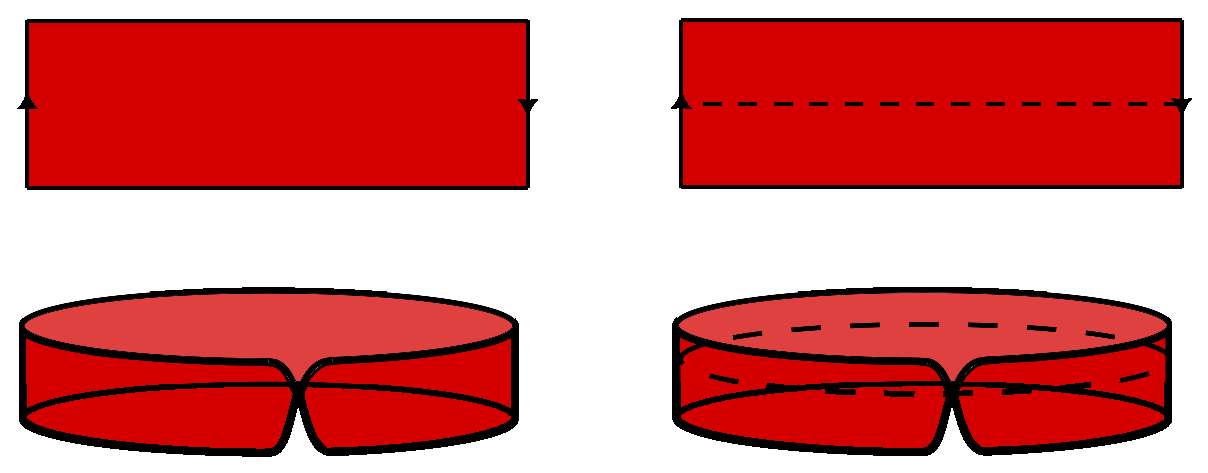
\includegraphics[scale=0.5]{Figures/Chapter1/mobius_band.eps}
                \caption{The M\"obius band obtained by identifying two sides of
                a rectangle.}
                \label{figure_1.6}
            \end{figure}
            Consider the ``core'' of the M\"obius band, signified by a dotted
            line in \ref{figure_1.6}. One cannot draw a curve above the core of
            the band, so this makes the surface nonorientable. The notion of
            Jacobians helps make sense of the intuitive notion of something
            being ``above'' an oriented surface.
    \end{enumerate}
\end{example}

\begin{definition}
    Let $M$ be a smooth manifold with orientations $(M,\{\phi_\a\})$ and
    $(M,\{\psi_\b\})$. We say the orientations \textbf{coincide} on a subset
    if the transition map $\phi_\a \circ \inv{\psi_\b}$ is defined on that
    subset, and has Jacobian with positive determinant. We say that the
    orientations \textbf{differ} on a subset if the orientation $\phi_\a \circ
    \inv{\psi_\b}$ is defined on that subset, and has Jacobian with negative
    determinant.
\end{definition}

\begin{definition}
    Let $M$ be an orientable manifold with orientation $(M,\{\phi_\a\})$. Where
    $\phi_\a:U_\a \xrightarrow{} \R^n$ is defined by $\phi_\a(x)=(x_1, \dots,
    x_n)$. We define the \textbf{opposite orientation} of $M$ to be the
    orientation $(M,\{\psi_\a\})$ where $\psi_\a:U_\a \xrightarrow{} \R^n$ is
    defined by $\psi_\a(x)=(-x_1, \dots, x_n)$. We denote $M$ with the
    orientation $(M,\{\psi_\a\})$ by $-M$.
\end{definition}

\begin{definition}
    If $M$ is an orientable manifold with boundary, we define the
    \textbf{induced orientation} on $\partial{M}$ to be the natural orientation
    on $\partial{M}$.
\end{definition}

\begin{definition}
    Let $M$ and  $N$ be smooth orientable manifolds of the same dimension with
    orientations $(M,\{\phi_\a\})$ and $(N,\{\psi_\b\})$. We call a smooth map
    $h:M \xrightarrow{} N$ \textbf{orientation preserving} if the Jacobians on
    all the maps $\psi_\b \circ h \circ \inv{\phi_a}$ have positive determinant
    wherever defined. If the Jacobians of all $\psi_\b \circ h \circ
    \inv{\phi_a}$ have negative determinant, we call $h$  \textbf{orientation
    reversing}.
\end{definition}

\begin{example}\label{example_1.10}
    \begin{enumerate}
        \item[(1)] The map $f:S^1 \xrightarrow{} S^1$ given by $f(\exp{2i\pi
            x})=\exp{4i\pi x}$ is orientation preserving, while the map $g:S^1
            \xrightarrow{} S^1$ given by $g(\exp{2i\pi x})=\exp{-2i\pi x}$ is
            orientation reversing.
    \end{enumerate}
\end{example}

\begin{definition}
    Let $M$ be a smooth manifold, and  $c$ a  $1$-dimensional submanifold of
    $M$. If there exists an atlas of  $M$ for which the charts that meet  $c$
    have Jacobians with positive determinant, then we call  $c$ an
    \textbf{orientation preserving} closed $1$-dimensional submanifold.
    Otherwise, if the Jacobians have negative determinant, we call $c$ an
    \textbf{orientation reversing} closed $1$-dimensional submanifold.
\end{definition}

\begin{lemma}\label{1.3.1}
    A manifold $M$ is nonorientable if, and only if  $M$ contains an orientation
    reversing closed  $1$-dimensional submanifold.
\end{lemma}
